%%%%%%%%%%%%%%%%%%%%%%%%%%%%%%%%%%%%%%%%%%%%%%%%%%%%%%%%%%%%%%%%
%                         My Template:                         %
%%%%%%%%%%%%%%%%%%%%%%%%%%%%%%%%%%%%%%%%%%%%%%%%%%%%%%%%%%%%%%%%

%Code(C++): \begin{lstlisting}
%Algorithm:
%\begin{breakablealgorithm}
%  \caption{?statement}
%  \begin{algorithmic}[?number]
%    \Require ?input
%    \Ensure ?output
%    \Procedure{Equal}{?parameters}
%      \State ?blabla
%    \EndProcedure
%  \end{algorithmic}
%\end{breakablealgorithm}

%Itemlisting: \begin{itemize} or \begin{enumerate}[label=(\alph*)]

%Math equation: \begin{align*}

%Table: \begin{tabular}{|c|c|c|}
%           blabla | blabla | blabla \\
%           ......
%Picture: \centerline{\includegraphics[scale=X]{FileName}

%%%%%%%%%%%%%%%%%%%%%%%%%%%%%%%%%%%%%%%%%%%%%%%%%%%%%%%%%%%%%%%%
%                         Title START!                         %
%%%%%%%%%%%%%%%%%%%%%%%%%%%%%%%%%%%%%%%%%%%%%%%%%%%%%%%%%%%%%%%%
\documentclass[11pt, a4paper, UTF8]{ctexart}
\usepackage{tikz}
\usetikzlibrary{shapes.geometric, arrows}

%%%%%%%%%%%%%%%%%%%%%%%%%%%%%%%%%%%
% File: preamble.tex
%%%%%%%%%%%%%%%%%%%%%%%%%%%%%%%%%%%
\usepackage{geometry}
\geometry{left = 1cm, right = 1cm, top = 1.5cm, bottom = 1.5cm}

\ProvidesPackage{zhfontcfg}
\usepackage{fontspec,xunicode}
\usepackage{xeCJK}
\usepackage{CJKutf8}
\usepackage{enumerate}
\defaultfontfeatures{Mapping=tex-text}
\XeTeXlinebreaklocale "zh"
\XeTeXlinebreakskip = 0pt plus 1pt minus 0.1pt
% Set fonts commands
% \newcommand\fontnamehei{文泉驿正黑}
% \newcommand\fontnamesong{文鼎PL新宋}
% \newcommand\fontnamekai{AR PL UKai CN}
% \newcommand\fontnamemono{Bitstream Vera Sans Mono}
% \newcommand\fontnameroman{Bitstream Vera Serif}
% \newcommand{\song}{\fontnamesong}
% \newcommand{\hei}{\fontnamehei}
% \newfontinstance\KAI {\fontnamekai}
% \newcommand{\kai}{\fontnamekai}
% \newCJKfontfamily\kai{FandolKai-Regular.otf}
% \newCJKfontfamily\hei{FandolHei-Regular.otf}
% \newCJKfontfamily\song{FandolSong-Regular.otf}
% \newCJKfontfamily\fang{FandolFang-Regular.otf}
% \setCJKfamilyfont{song}[BoldFont=FandolSong-Bold.otf]{FandolSong-Regular.otf}
% \setCJKfamilyfont{hei}{FandolHei-Regular.otf}
% \setCJKfamilyfont{kai}{FandolKai-Regular.otf}
\newcommand{\song}{\CJKfamily{song}}
\newcommand{\hei}{\CJKfamily{hei}}
\newcommand{\kai}{\CJKfamily{kai}}
\newcommand{\fs}{\CJKfamily{fs}}
\newcommand{\tqs}{\textquotesingle}

\defaultfontfeatures{
    Path = /usr/local/texlive/2018/texmf-dist/fonts/opentype/public/fontawesome/ }
\usepackage{fontawesome}
\newcommand{\me}[2]{\author{{\bfseries 姓名:}\underline{#1}\hspace{2em}{\bfseries 学号:}\underline{#2}}}

% Always keep this.
\newcommand{\noplagiarism}{
    \begin{center}
        \fbox{\begin{tabular}{@{}c@{}}
            请独立完成作业,不得抄袭。\\
            若参考了其它资料,请给出引用。\\
            鼓励讨论,但需独立书写解题过程。
        \end{tabular}}
    \end{center}
}

% Each hw consists of three parts:
% (1) this homework
\newcommand{\beginthishw}{\part{作业\faTasks}}
% (2) corrections (Optional)
\newcommand{\begincorrection}{\part{订正\faRefresh}}
% (3) any feedback (Optional)
\newcommand{\beginfb}{\part{反馈\faShareSquareO}}

% For math
\usepackage{amsmath}
\usepackage{amsfonts}
\usepackage{amssymb}
\usepackage{graphicx}
\usepackage{listings}
\usepackage{xcolor}
\usepackage{clrscode3e}
\usepackage{enumitem}
\usepackage{tikz}
\usepackage{tabularx}
\usepackage{multirow}
\newcolumntype{Y}{>{\centering\arraybackslash}X}
\newcolumntype{P}{>{\centering\arraybackslash}p}
%bigger integrate symbol
\usepackage{exscale}
\usepackage{relsize}
\usepackage{textcomp}

% colors
\newcommand{\red}[1]{\textcolor{red}{#1}}
\newcommand{\blue}[1]{\textcolor{blue}{#1}}
\newcommand{\teal}[1]{\textcolor{teal}{#1}}

% algorithms
\usepackage[]{algorithm}
\usepackage[noend]{algpseudocode} % noend
\makeatletter
\newenvironment{breakablealgorithm}
  {% \begin{breakablealgorithm}
      \begin{center}
          \refstepcounter{algorithm}% New algorithm
          \hrule height.8pt depth0pt \kern2pt% \@fs@pre for \@fs@ruled 画线
          \renewcommand{\caption}[2][\relax]{% Make a new \caption
              {\raggedright\textbf{\ALG@name~\thealgorithm} ##2\par}%
          \ifx\relax##1\relax % #1 is \relax
          \addcontentsline{loa}{algorithm}{\protect\numberline{\thealgorithm}##2}%
          \else % #1 is not \relax
          \addcontentsline{loa}{algorithm}{\protect\numberline{\thealgorithm}##1}%
          \fi
          \kern2pt\hrule\kern2pt
          }
          }{% \end{breakablealgorithm}
              \kern2pt\hrule\relax% \@fs@post for \@fs@ruled 画线
  \end{center}
  }
\makeatother
\renewcommand{\algorithmicrequire}{\textbf{Input:}} % Use Input in the format of Algorithm
\renewcommand{\algorithmicensure}{\textbf{Output:}} % Use Output in the format of Algorithm
% See [Adjust the indentation whithin the algorithmicx-package when a line is broken](https://tex.stackexchange.com/a/68540/23098)
\newcommand{\algparbox}[1]{\parbox[t]{\dimexpr\linewidth-\algorithmicindent}{#1\strut}}
\newcommand{\hStatex}[0]{\vspace{5pt}}
\makeatletter
\newlength{\trianglerightwidth}
\settowidth{\trianglerightwidth}{$\triangleright$~}
\algnewcommand{\LineComment}[1]{\Statex \hskip\ALG@thistlm \(\triangleright\) #1}
\algnewcommand{\LineCommentCont}[1]{\Statex \hskip\ALG@thistlm%
  \parbox[t]{\dimexpr\linewidth-\ALG@thistlm}{\hangindent=\trianglerightwidth \hangafter=1 \strut$\triangleright$ #1\strut}}
\makeatother


% Define theorem-like environments
\usepackage[amsmath, thmmarks, framed]{ntheorem}
\usepackage{framed}

\theoremheaderfont{\kai\bfseries}
\theoremstyle{break}
\theorembodyfont{\song}
% \theorembodyfont{\kai}
\theoremseparator{\vspace{1mm}}
\renewcommand*\FrameCommand{{\color{gray}\vrule width 3pt \hspace{10pt}}}
\newframedtheorem{problem}{\faCheckSquareO \ Problem}

\theorempostwork{\hrule}
\newtheorem*{solution}{\faEdit \ Solution}
\newtheorem*{revision}{\faEdit \ Revision}

\theoremstyle{plain}
\newtheorem*{cause}{\faCoffee \ Cause}
\newtheorem*{remark}{\faCommentingO \ Remark}

\theoremstyle{break}
\theoremsymbol{\ensuremath{\Box}}
\newtheorem*{proof}{\faEdit \ Proof}

\renewcommand\figurename{Figure}
\renewcommand\tablename{Table}

%enumeration
\setenumerate[1]{
    itemsep=0pt,
partopsep=0pt,
parsep=\parskip,
topsep=0pt,
leftmargin=20pt
}
\setitemize[1]{
    itemsep=0pt,
partopsep=0pt,
parsep=\parskip,
topsep=0pt,
leftmargin=20pt
}
\setdescription{
    itemsep=0pt,
partopsep=0pt,
parsep=\parskip,
topsep=0pt,
leftmargin=20pt
}
\lstset{
    language={[ISO]C++},
numbers=left,
numberstyle= \tiny,
commentstyle=\color{red!50!green!50!blue!50},
rulesepcolor=\color{red!20!green!20!blue!20},
keywordstyle=\color{blue!90}\bfseries,
showstringspaces=false,
stringstyle=\ttfamily,
}

% For figures
% for fig with caption: #1: width/size; #2: fig file; #3: fig caption
\newcommand{\fig}[3]{
    \centerline{\includegraphics[scale=#1]{#2}}
    \centerline{#3}
}

% for fig without caption: #1: width/size; #2: fig file
\newcommand{\fignc}[2]{
    \centerline{\includegraphics[scale=#1]{#2}}
}



\title{Homework 5}
\me{毕秋宇}{171860624}
\date{\today}

\begin{document}
\thispagestyle{empty}
\maketitle
% \noplagiarism

%%%%%%%%%%%%%%%%%%%%%%%%%%%%%%%%%%%%%%%%%%%%%%%%%%%%%%%%%%%%%%%%
%                       Homework START!                        %
%%%%%%%%%%%%%%%%%%%%%%%%%%%%%%%%%%%%%%%%%%%%%%%%%%%%%%%%%%%%%%%%
\beginthishw
%%%%%%%%%%%%%%%%%%%%
\begin{problem}[Naive Bayes Classifier]
    We learned about the naive Bayes classifier using the "property conditional independence hypothesis". Now we have a data set as shown in the following table:

    % \begin{table}[htp]
    % \label{tab:aStrangeTable}
    % \caption{Dataset}
    \begin{tabular}{c|ccccc}
        % \centering
        \hline
        & $x_1$ & $x_2$ & $x_3$ & $x_4$ & $y$ \\
        \hline
        Instance1   & 1 & 1 & 1 & 0 & 1 \\
        \hline
        Instance2   & 1 & 1 & 0 & 0 & 0 \\
        \hline
        Instance3   & 0 & 0 & 1 & 1 & 0 \\
        \hline
        Instance4   & 1 & 0 & 1 & 1 & 1 \\
        \hline
        Instance5   & 0 & 0 & 1 & 1 & 1 \\
        \hline
    \end{tabular}
    % \end{table}
    \

    \begin{enumerate}
        \item[(1)][10pts]  Calculate: $\Pr\{ y=1 | \mathbf{x}=(1,1,0,1) \}$ and $\Pr\{ y=0 | \mathbf{x}=(1,1,0,1) \}$.
        \item[(2)][10pts] After using Laplacian Correction, recalculate the value in the previous question.
    \end{enumerate}
\end{problem}

%\begin{remark}

%\end{remark}

\begin{solution}
    \begin{enumerate}
        \item[(1)]
            \[\Pr\{y=1|\mathbf{x}=(1,1,0,1)\}=\frac{\Pr\{y=1,x=(1,1,0,1)\}}{\Pr\{x=(1,1,0,1)\}}\]
            \[=\Pr\{y=1\}\times\Pr\{y=1|x_1=1\}\times\Pr\{y=1|x_2=1\}\times\Pr\{y=1|x_3=0\}\times\Pr\{y=1|x_4=1\}\]
            \[=\frac{3}{5}\times\frac{2}{3}\times\frac{1}{2}\times0\times\frac{2}{3}=0\]
            \[\Pr\{y=0|\mathbf{x}=(1,1,0,1)\}=\frac{\Pr\{y=0\}\Pr\{\mathbf{x}=(1,1,0,1)|y=0\}}{\Pr\{\mathbf{x}=(1,1,0,1)\}}\]
            \[=\Pr\{y=0\}\times\Pr\{\mathbf{x}^{\prime}_{1}=\mathbf{x}_1|y=0\}\times\Pr\{\mathbf{x}^{\prime}_2=\mathbf{x}_2|y=0\}\times\Pr\{\mathbf{x}^{\prime}_3=\mathbf{x}_3|y=0\}\times\Pr\{\mathbf{x}^{\prime}_4=\mathbf{x}_4|y=0\}\]
            \[=\frac{2}{5}\times\frac{1}{2}\times\frac{1}{2}\times\frac{1}{2}\times\frac{1}{2}=\frac{1}{40}\]
        \item[(2)] Using the Laplacian correction, we get that
            \[\hat{\Pr}\{y=1|\mathbf{x}=(1,1,0,1)\}=\frac{\hat{\Pr}\{y=1,x=(1,1,0,1)\}}{\hat{\Pr}\{x=(1,1,0,1)\}}\]
            \[=\hat{\Pr}\{y=1\}\times\hat{\Pr}\{y=1|x_1=1\}\times\hat{\Pr}\{y=1|x_2=1\}\times\hat{\Pr}\{y=1|x_3=0\}\times\hat{\Pr}\{y=1|x_4=1\}\]
            \[=\frac{4}{7}\times\frac{3}{5}\times\frac{2}{5}\times\frac{1}{5}\times\frac{3}{5}=\frac{72}{4375}\]
            \[\hat{\Pr}\{y=0|\mathbf{x}=(1,1,0,1)\}=\frac{\hat{\Pr}\{y=0\}\hat{\Pr}\{\mathbf{x}=(1,1,0,1)|y=0\}}{\hat{\Pr}\{\mathbf{x}=(1,1,0,1)\}}\]
            \[=\hat{\Pr}\{y=0\}\times\hat{\Pr}\{\mathbf{x}^{\prime}_{1}=\mathbf{x}_1|y=0\}\times\hat{\Pr}\{\mathbf{x}^{\prime}_2=\mathbf{x}_2|y=0\}\times\hat{\Pr}\{\mathbf{x}^{\prime}_3=\mathbf{x}_3|y=0\}\times\hat{\Pr}\{\mathbf{x}^{\prime}_4=\mathbf{x}_4|y=0\}\]
            \[=\frac{3}{7}\times\frac{1}{2}\times\frac{1}{2}\times\frac{1}{2}\times\frac{1}{2}=\frac{3}{112}\]
    \end{enumerate}
\end{solution}
%%%%%%%%%%%%%%%%%%%%%
\begin{problem}[Bayes Optimal Classifier]
    For a binary classification task, when data in the two classes satisfies Gauss distribution and have the same variance, please prove that LDA can produce the bayes optimal classifier.
\end{problem}

%\begin{remark}

%\end{remark}

\begin{solution}
    By the definition of Gauss distribution, we get that $f_{c}(x)=\frac{e^{-\frac{(x-\mu)^{T}(x-\mu)}{2\Sigma}}}{\sqrt{(2\pi)^d|\Sigma|}}$\\
    Where $\Sigma$ is the covariance matrix, $\mu$ is the mean vector.\\
    So we can get that the bayes optimal classifier satisfies \[h(x)=\arg\max_{c}\Pr\{c|x\}=\arg\max_{c}\Pr\{c\}f_{c}(x)\]
    The boundary between two classes is $\Pr\{c_1\}f_{c_{1}}(x)=\Pr\{c_2\}f_{c_2}f_{c_2}(x)$.\\
    Bring the function above and take the logarithm of both sides we get that the boundary is
    \[\log(\Pr\{c_1\})-\frac{(x-\mu_{c_1})^{T}(x-\mu_{c_1})}{2\Sigma} = \log(\Pr\{c_2\})-\frac{(x-\mu_{c_2})^{T}(x-\mu_{c_2})}{2\Sigma}\]
    That is to say,
    \[\log(\frac{\Pr\{c_1\}}{\Pr\{c_2\}})=\frac{(x-\mu_{c_1})^{T}(x-\mu_{c_1})-(x-\mu_{c_2})^{T}(x-\mu_{c_2})}{2\Sigma}\]
    So we get that
    \[\log(\frac{\Pr\{c_1\}}{\Pr\{c_2\}})=\frac{x^{T}x-2x^{T}\mu_{c_1}+\mu_{c_1}^{T}\mu_{c_1}-x^{T}x+2x^{T}\mu_{c_2}-\mu_{c_2}^{T}\mu_{c_2}}{2\Sigma}=\frac{2x^{T}(\mu_{c_2}-\mu_{c_1})+\mu^{T}_{c_1}\mu_{c_1}-\mu^{T}_{c_2}\mu_{c_2}}{2\Sigma}\]
    That is
    \[2\log(\frac{\Pr\{c_1\}}{\Pr\{c_2\}})-2x^{T}\Sigma^{-1}(\mu_{c_2}-\mu_{c_1})-\mu^{T}_{c_1}\Sigma^{-1}\mu_{c_1}+\mu^{T}_{c_2}\Sigma^{-1}\mu_{c_2}\]
    From LDA method, we know $w=\Sigma^{-1}(\mu_{c_1}-\mu_{c_2})$ in the target function $w^{T}x+b$, it is same as we get from bayes optimal classifier.\\
    Finally, we proved that LDA can produce the bayes optimal classifier.
\end{solution}
%%%%%%%%%%%%%%%%%%%%%
\begin{problem}[Ensemble Methods in Practice]
    Due to their outstanding performance and robustness, ensemble methods are very popular in machine community. In this experiment we will practice ensemble learning methods based on two classic
    ideas: Boosting and Bagging.

    In this experiment, we use an UCI dataset Adult. You can refer to the link\footnote{http://archive.ics.uci.edu/ml/datasets/Adult} to see the data description and download the dataset.

    Adult is an class imbalanced dataset, so we select AUC as the performance measure. You can adopt sklearn to calculate AUC.

    (1) [10pts] You need finish the code in Python, and only have two files: AdaBoost.py, RandomForestMain.py. (The training and testing process are implemented in one file for each algorithm.)

    (2) [40pts] The is experiment requires to finish the following methods:

    \begin{enumerate}
        \item Implement AdaBoost algorithm according to the Fig(8.3), and adopt decision tree as the base learner (For the base learner, you can import sklearn.)
        \item  Implement Random Forest algorithm. Please give a pseudo-code in the experiment report.
        \item According to the AdaBoost and random forest, analysis the effect of the number of base learners on the performance. Specifically, given the number of base learners, use 5-fold cross validation to obtain the AUC. The range of the number of base learners is decided by yourself.
        \item Select the best number of base classifiers for AdaBoost and random forests, and obtain the AUC in the test set.
    \end{enumerate}

    (3) [10pts] In the experimental report, you need to present the detail experimental process. The experimental report needs to be hierarchical and organized, so that the reader can understand the purpose, process and result of the experiment.

\end{problem}

%\begin{remark}

%\end{remark}

\begin{solution}
    \begin{enumerate}
        \item[(1)] Two files are in the same folders.
        \item[(2)] The pseudo-code of Random Forest algorithm are as follows:
            \begin{algorithm}
                \caption {\textsc{Random Forest}}
                \begin {algorithmic}[1] % 每行显示行号
                \Require $X_{train}$ ,$y_{train}$
                \Ensure $Model$
                \Function {Fit}{$X_{train}, y_{train}$}
                \State
                \For{$tree$ in $forest$}
                \State{$idx = randsamp(X_{train}.features)$}
                \State$x_{train} = X_{train}[idx]$
                \State$tree.fit(x_{train})$
                \State
                \Return{$model$}
                % \EndFor
                \EndFunction
            \end{algorithmic}
    \end{algorithm}
\item[(3)]
    Firstly, I download the "adult.data" and "adult.test" files and then use read csv function to read the data.

    However, the data exists deficiency and string value, so I use fillna and getdummies to convert it to the workable data. When preprocessing the string values, I find that the types of test file are different from the train file, so I concat those two DataFrame using getdummies function and then split it to the original size.

    And then, I create AdaBoost and RandomForest algorithm using the DecisionTreeRegresser from sklearn. I choose DecisionTreeRegresser other than DecisionTreeClassigier because I need to calculate the AUC value. In the predict part, if regression value is bigger than $0.5$ we decide it as positive, we decide it as negative otherwise.

    Last but not least, I need to decide the hype-parameters in AdaBoost and RandomForest algorithm. I use gridsearchCV function to select the best values.

    The final AUC are as follows:
    \begin{figure}[H]
        \centering
        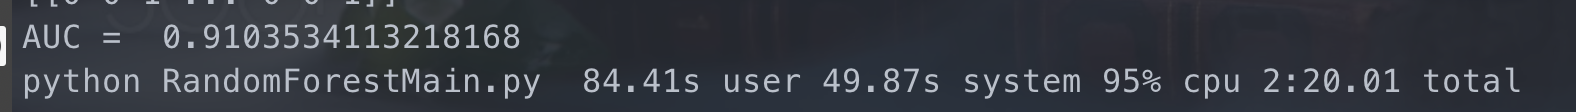
\includegraphics[width=0.7\linewidth]{1.png}
        \caption{AUC of RandomForest}
        \label{fig:Random}
    \end{figure}
    \begin{figure}[H]
        \centering
        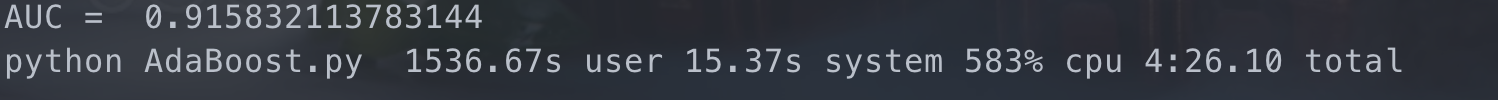
\includegraphics[width=0.7\linewidth]{2.png}
        \caption{AUC of AdaBoost}
        \label{fig:Random}
    \end{figure}
    And the number of weak classifiers is 2000, the number of estimators is 2000, min samples split is 2, min impurity decrease is 0 and splitter is random.
\end{enumerate}
\end{solution}
%%%%%%%%%%%%%%%%%%%%%
% \begin{problem}[Principal Component Analysis]
% \end{problem}

%\begin{remark}

%\end{remark}

% \begin{solution}
% \end{solution}
%%%%%%%%%%%%%%%%%%%%%
% \begin{problem}[TC 32.3-3]
% \end{problem}

%\begin{remark}

%\end{remark}

% \begin{solution}
%
% \end{solution}
%%%%%%%%%%%%%%%%%%%%
%\newpage
%%%%%%%%%%%%%%%%%%%%


%%%%%%%%%%%%%%%%%%%%%%%%%%%%%%%%%%%%%%%%%%%%%%%%%%%%%%%%%%%%%%%%
%                      Correction START!                       %
%%%%%%%%%%%%%%%%%%%%%%%%%%%%%%%%%%%%%%%%%%%%%%%%%%%%%%%%%%%%%%%%
\begincorrection
%%%%%%%%%%%%%%%%%%%%
%\begin{problem}[]

%\end{problem}

%\begin{cause}
%
%\end{cause}

%\begin{revision}

%\end{revision}
%%%%%%%%%%%%%%%%%%%%
%\newpage
%%%%%%%%%%%%%%%%%%%%


%%%%%%%%%%%%%%%%%%%%%%%%%%%%%%%%%%%%%%%%%%%%%%%%%%%%%%%%%%%%%%%%
%                       Feedback START!                        %
%%%%%%%%%%%%%%%%%%%%%%%%%%%%%%%%%%%%%%%%%%%%%%%%%%%%%%%%%%%%%%%%
\beginfb
%\begin{itemize}
%
%\end{itemize}


%%%%%%%%%%%%%%%%%%%%%%%%%%%%%%%%%%%%%%%%%%%%%%%%%%%%%%%%%%%%%%%%
%                        Homework END!                         %
%%%%%%%%%%%%%%%%%%%%%%%%%%%%%%%%%%%%%%%%%%%%%%%%%%%%%%%%%%%%%%%%
\end{document}

